\documentclass[convert]{standalone}

\usepackage{tikz}
\usepackage{graphicx}
\pagestyle{empty}

% INT_AY20_MP3_L24-Charge-in-field-01.png

\begin{document}
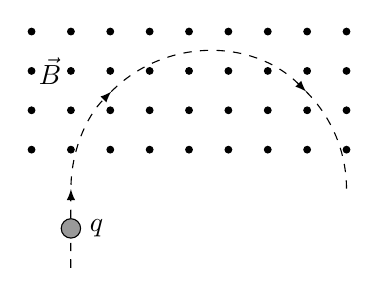
\begin{tikzpicture}[> = latex]

	% Definitions
	
	\def\lattice{0.5}		% Lattice spacing for magnetic field dots
	\def\xmax{9}		% x dimension of bounding box in lattice spacings
	\def\ymax{4}		% y dimension of bounding box in lattice spacings

	
	% Magnetic field
	
	% Each magnetic field indicator is placed in lattice with \lattice spacing,
	% starting \lattice from bounding box
	
	\foreach \x in {1, 2, ..., \xmax}
	\foreach \y in {1, 2, ..., \ymax}
		\filldraw (\x * \lattice, \y * \lattice) circle (1.2 pt);
		
		
	% Trajectory of ion, and ion itself
	
	\begin{scope}[dashed, ->]
	
		\draw (2 * \lattice, -1) -- (2 * \lattice, 0);
		\draw (2 * \lattice, -1) -- (2 * \lattice, 0) arc (180 : 135 : {0.5 * \lattice * (\xmax - 2)}) coordinate (arc1);
		\draw (arc1) arc (135 : 45 : {0.5 * \lattice * (\xmax - 2)}) coordinate (arc2);
		
	\end{scope}
	
	\draw [dashed] (arc2) arc (45 : 0 : {0.5 * \lattice * (\xmax - 2)});				% Finish drawing trajectory w/o arrow
	\filldraw [fill = gray!80] (2 * \lattice, -0.5) circle (3.5 pt) node [right] {$~q$};		% Draw ion
	
	\filldraw [fill = white] (2 * \lattice, 1.5) circle (0.1 pt) node [left] {$\vec{B}$};	

\end{tikzpicture}
\end{document}